\section{Problem Set 8}

In this section, we go over the implementation of our Extended Kalman Filter (EKF) based on our prior description of the system architecture, provided in Section \ref{sec:7}. 

\subsection{Ground Truth Propagator}

Using GVEs, provide equations (or refer to existing equations)

\subsection{Generating Measurements}

Our measurement vector (abstracting away the information we get from vision, range and GPS), is a vector that includes noisy versions of the RTN and ECI positions of the deputies. 

\begin{align}
    y &= \begin{bmatrix}
        y_{SV2} \\
        y_{SV3}
    \end{bmatrix} \\
    &= \begin{bmatrix}
        \boldsymbol{r_{SV2}}^{RTN}\\
        \boldsymbol{r_{SV2}}^{ECI} \\
        \boldsymbol{r_{SV3}}^{RTN} \\
        \boldsymbol{r_{SV3}}^{ECI} \\
    \end{bmatrix}_{12\times 1}
\end{align}

To generate these measurements, we first take our true ECI and RTN positions of the deputy. These are calculated by taking the GVE-propagated orbital elements and converting them to RTN and ECI values of the deputy. Then, we add gaussian white noise $V_t$ to the true values to create the noisy measurements. The added noise $V_t$ for a single deputy is given by:

\begin{align}
    V_{t, SV3} = \mathcal{N}\left(0, \begin{bmatrix}
        10^{-3} I_3 \\
         I_3 \\
 \end{bmatrix}\right) km
\end{align}

Note that this noise is in kilometers, since the ECI and RTN values are in kilometers. Therefore, we set up our noise to have a variance $\sigma^2 = 1 m$

\subsection{Initializing Estimate Mean and Covariance}

We initialize the initial mean $\mu_0$ and the initial covariance $\Sigma_0$ in the following manner...

\subsection{EKF Implementation and Choice of Q and R}

EKF algorithm given below.

Q and R chosen to be the following values.

\subsection{EKF Results and Analysis}

\begin{figure}[H]
    \centering
    \begin{subfigure}[t]{0.49\textwidth}
        \centering
        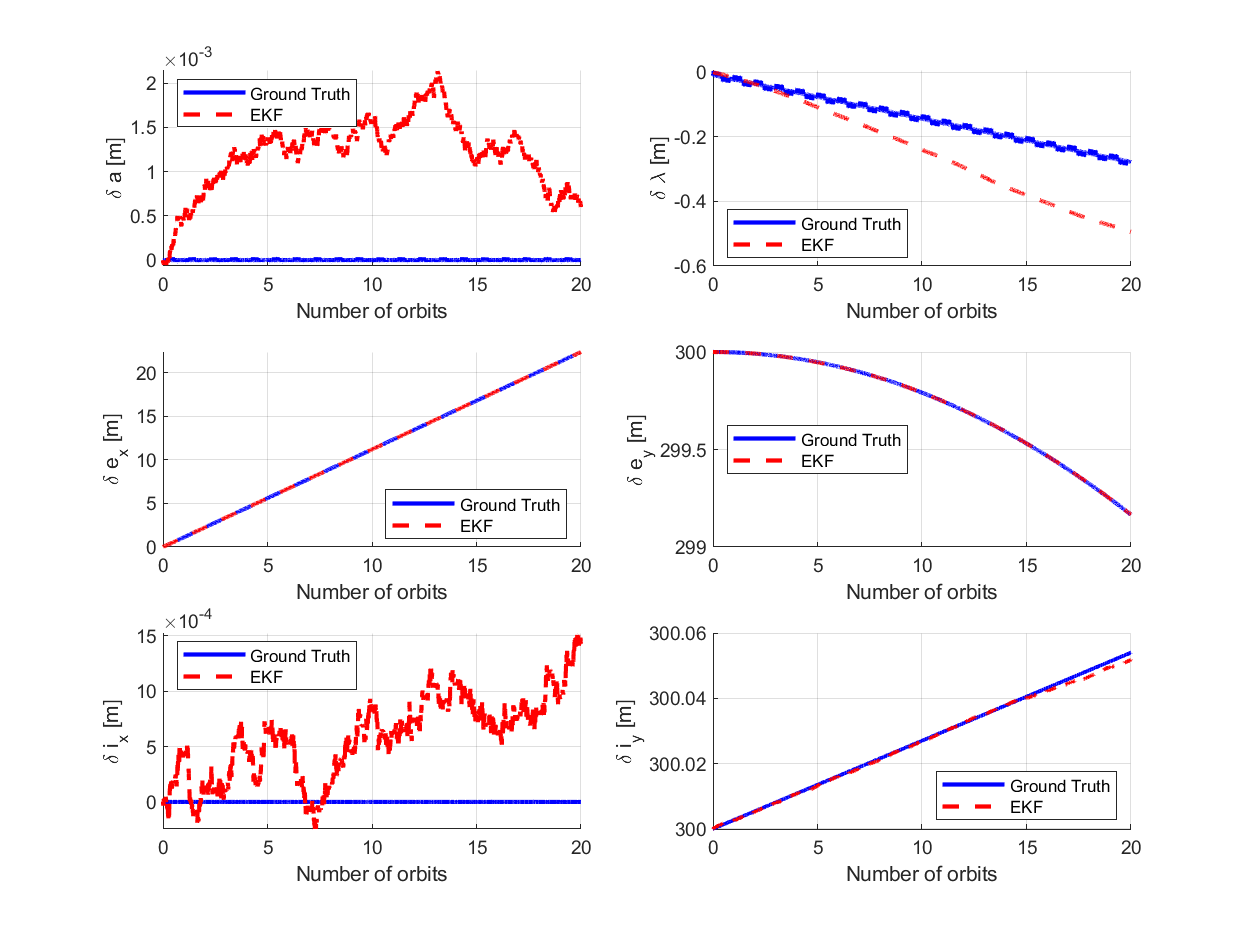
\includegraphics[width=\linewidth]{sim/figures/PS8/ROE_over_time_SV2_comparison.png}
        \caption{Ground Truth and EKF estimates for SV2 over time.}
        \label{fig:sv2_ekf_estimates}
    \end{subfigure}
    \hfill
    \begin{subfigure}[t]{0.49\textwidth}
        \centering
        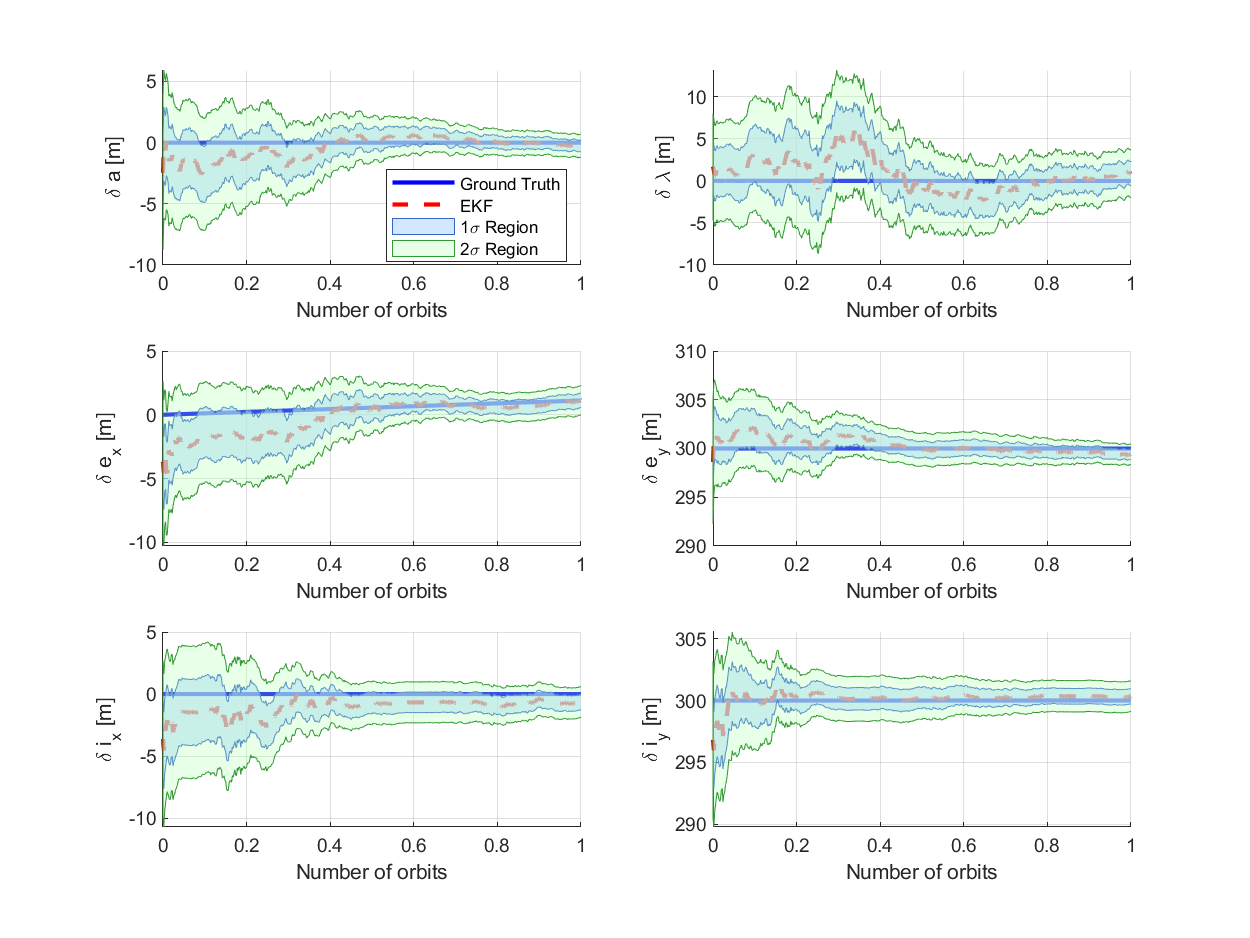
\includegraphics[width=\linewidth]{sim/figures/PS8/ROE_over_time_SV2_comparison_zoomed.png}
        \caption{Zoomed-in view over the first orbit showing convergence.}
        \label{fig:sv2_ekf_estimates_zoom}
    \end{subfigure}
    \caption{EKF estimation results for SV2.}
    \label{fig:sv2_ekf_combined}
\end{figure}

\begin{figure}[H]
    \centering
    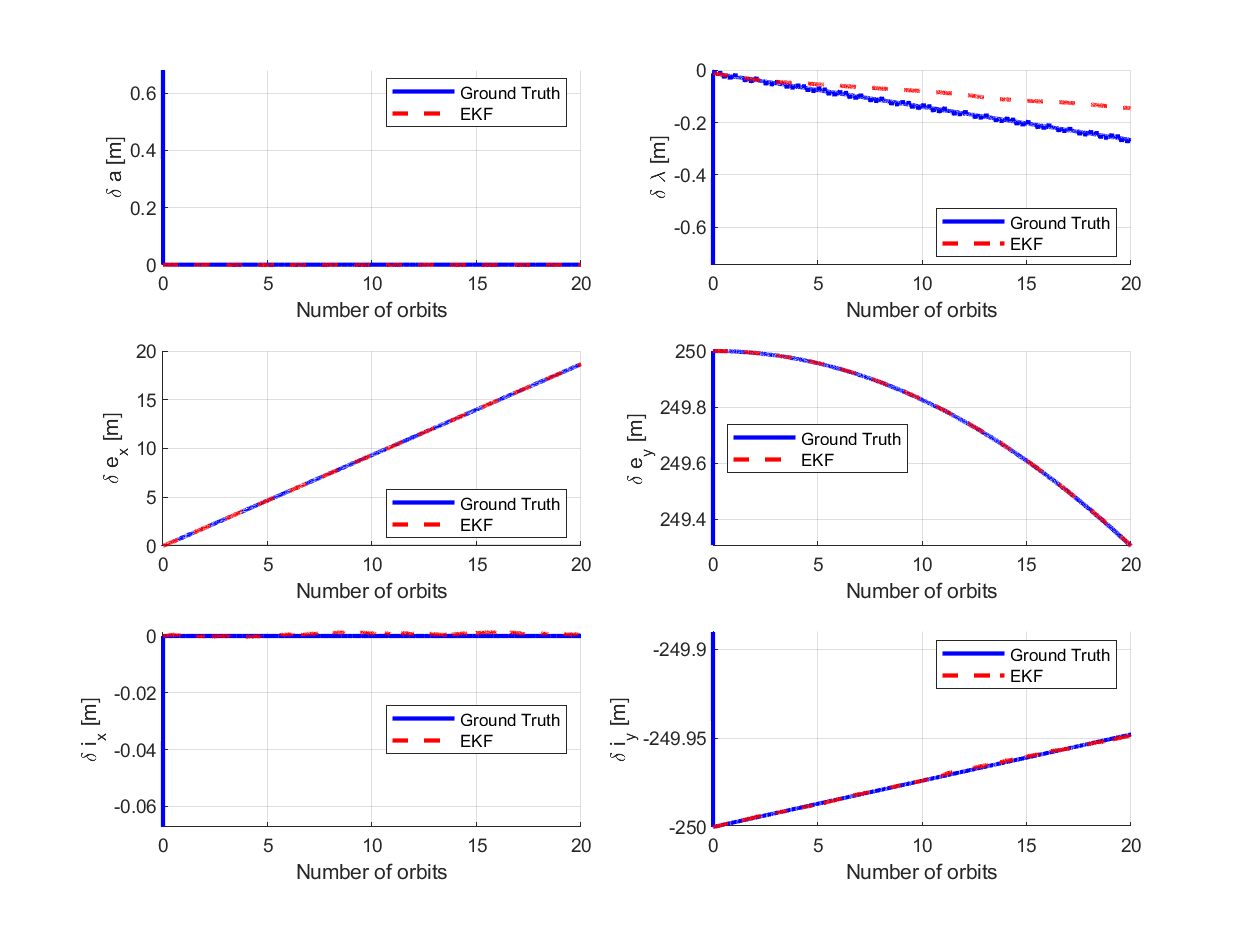
\includegraphics[width=0.7\linewidth]{sim/figures/PS8/ROE_over_time_SV3_comparison.png}
    \caption{Ground Truth and EKF estimates for SV3 over time}
    \label{fig:sv3_ekf_estimates}
\end{figure}

\begin{figure}[H]
    \centering
    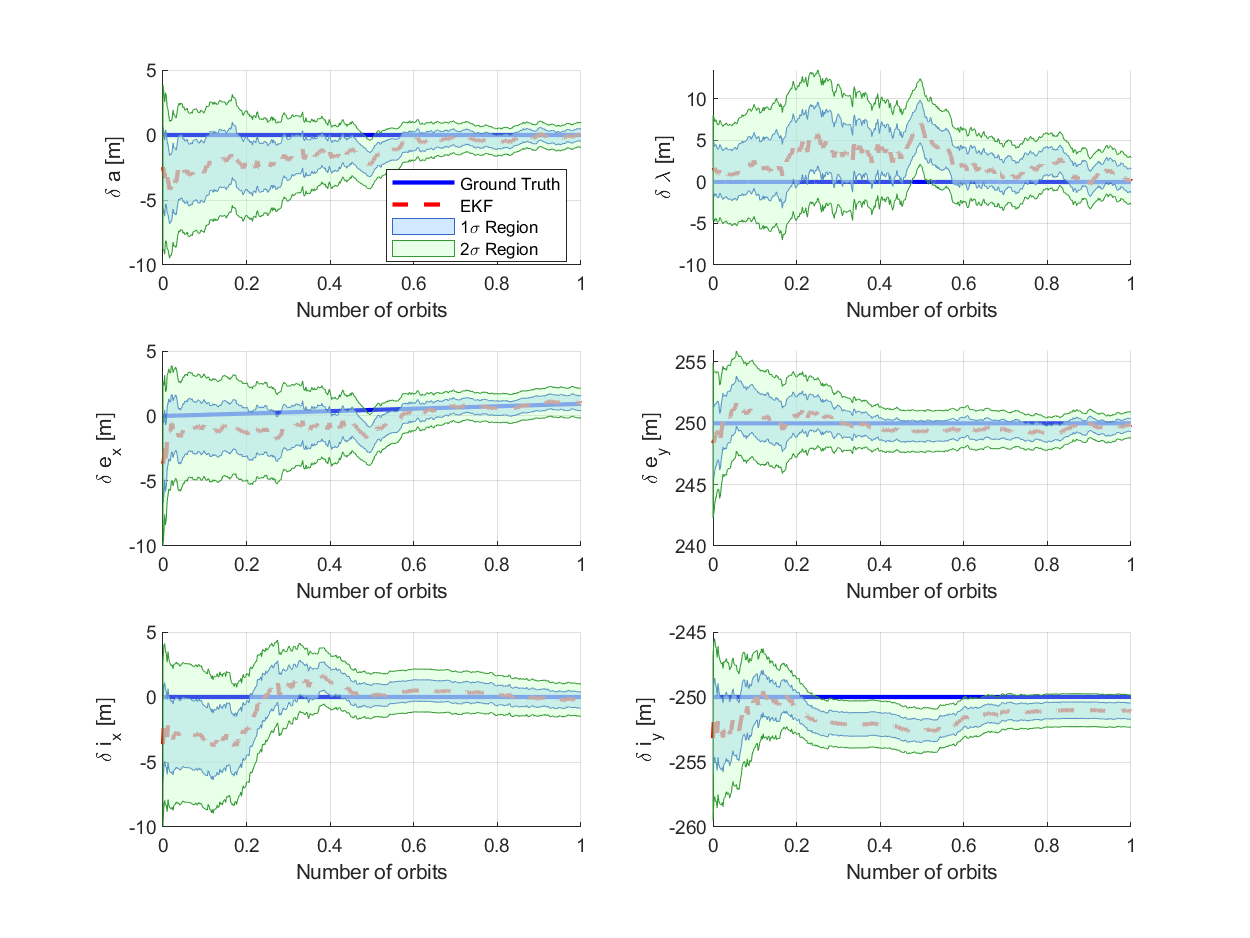
\includegraphics[width=0.7\linewidth]{sim/figures/PS8/ROE_over_time_SV3_comparison_zoomed.png}
    \caption{Ground Truth and EKF estimates for SV3, Zoomed version to first orbit, showing convergence.}
    \label{fig:sv3_ekf_estimates_zoom}
\end{figure}

\begin{figure}[H]
    \centering
    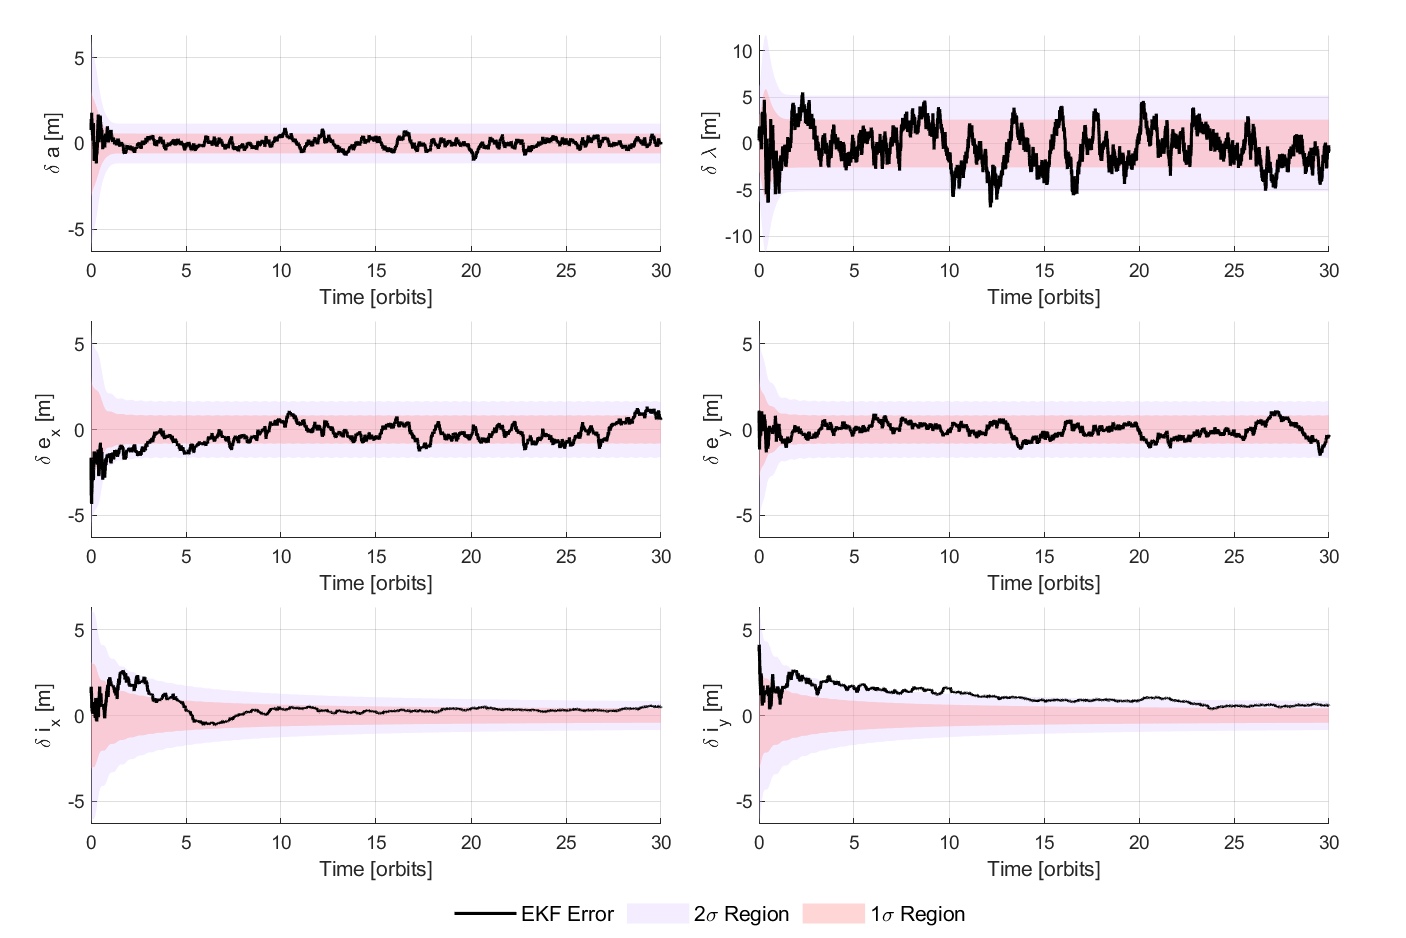
\includegraphics[width=0.7\linewidth]{sim/figures/PS8/EKF_error_SV2.png}
    \caption{Error in EKF estimates for SV2 over time}
    \label{fig:sv2_ekf_error}
\end{figure}

\begin{figure}[H]
    \centering
    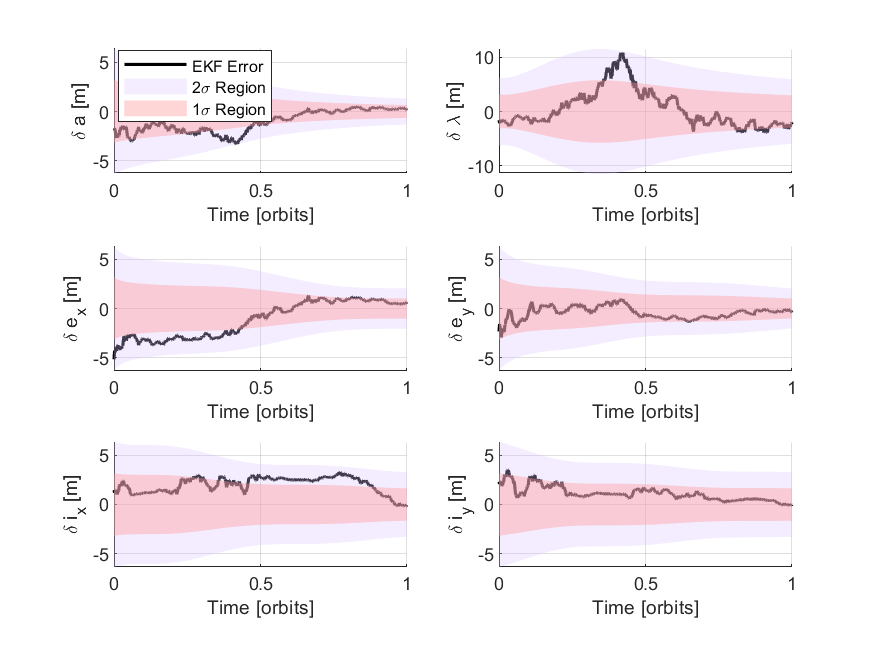
\includegraphics[width=0.7\linewidth]{sim/figures/PS8/EKF_error_SV2_zoomed.png}
    \caption{Error in EKF estimates for SV2 over time, zoomed to the first orbit to show convergence}
    \label{fig:sv2_ekf_error_zoomed}
\end{figure}

\begin{figure}[H]
    \centering
    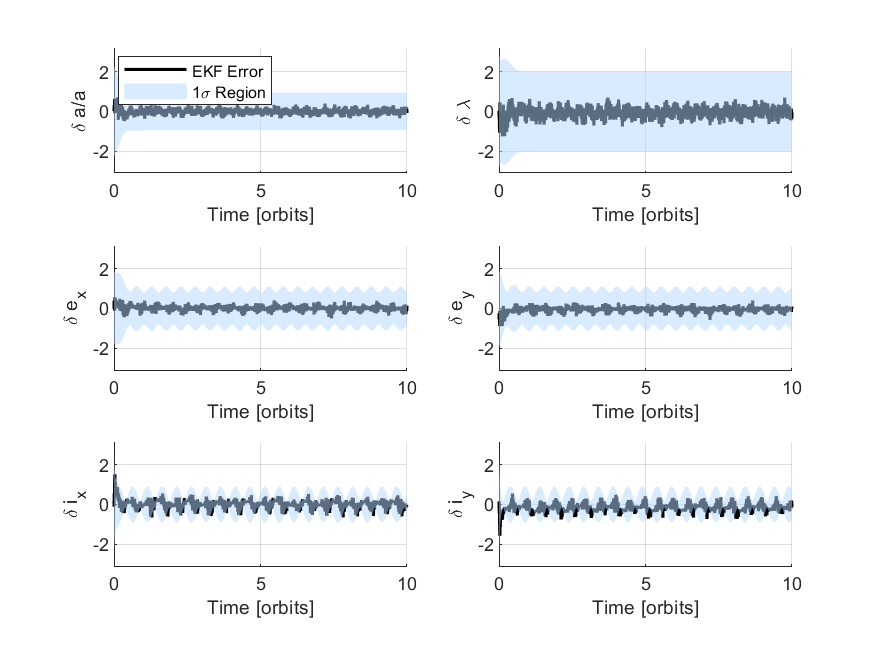
\includegraphics[width=0.7\linewidth]{sim/figures/PS8/EKF_error_SV3.png}
    \caption{Error in EKF estimates for SV3 over time}
    \label{fig:sv3_ekf_error}
\end{figure}

\begin{figure}[H]
    \centering
    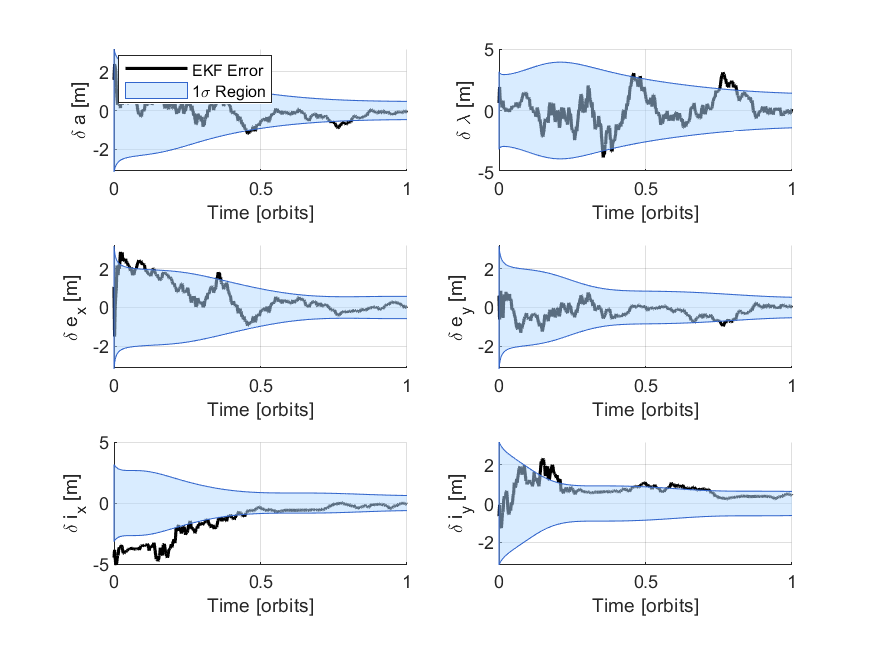
\includegraphics[width=0.7\linewidth]{sim/figures/PS8/EKF_error_SV3_zoomed.png}
    \caption{Error in EKF estimates for SV3 over time, zoomed to the first orbit to show convergence}
    \label{fig:sv3_ekf_error_zoomed}
\end{figure}


\begin{figure}[H]
    \centering
    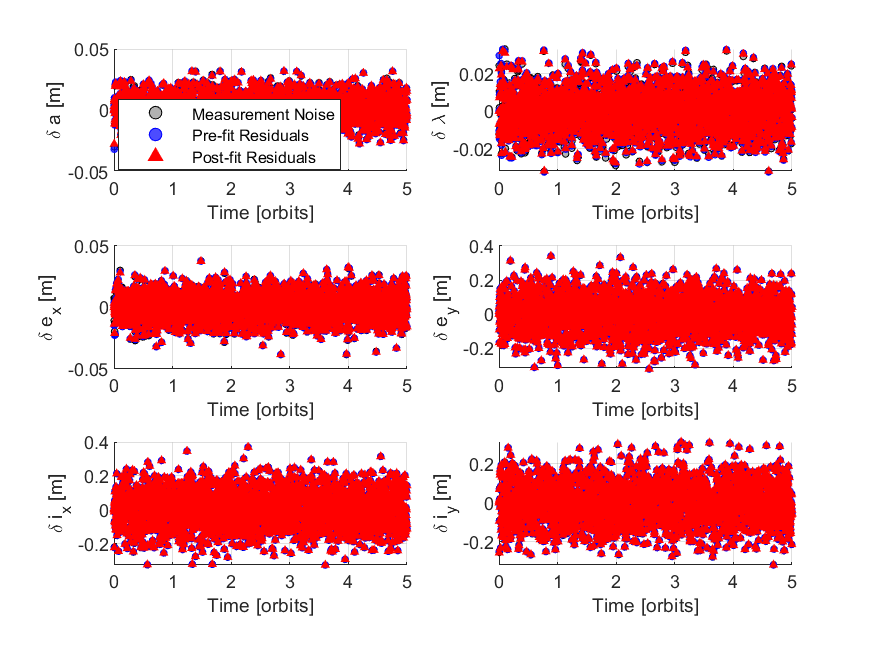
\includegraphics[width=0.7\linewidth]{sim/figures/PS8/residuals_SV2.png}
    \caption{Pre-fit and post-fit residuals in SV2}
    \label{fig:sv2_residuals}
\end{figure}

\begin{figure}[H]
    \centering
    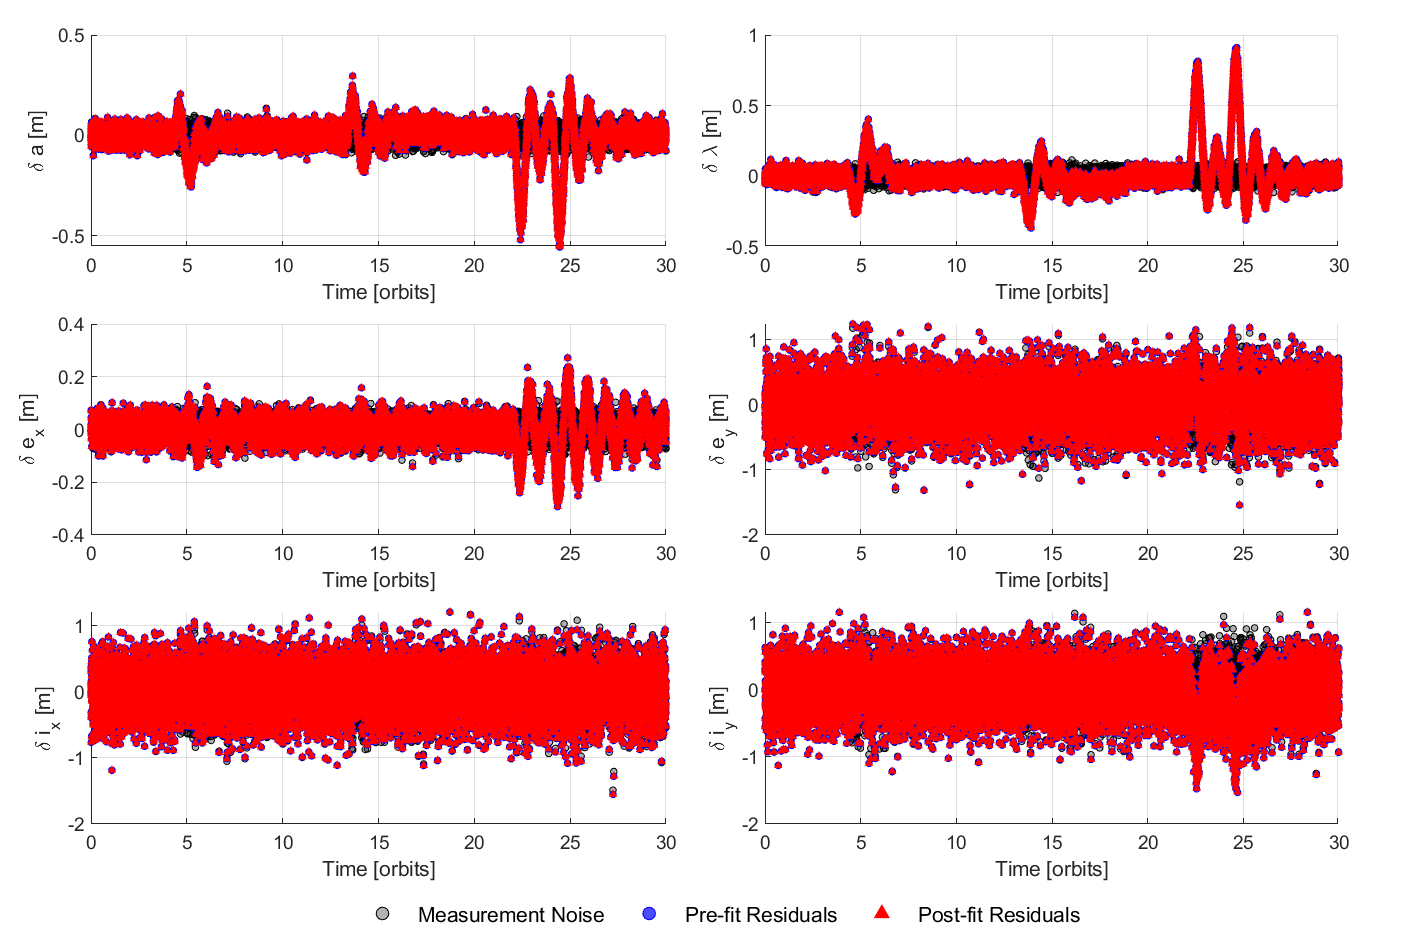
\includegraphics[width=0.7\linewidth]{sim/figures/PS8/residuals_SV3.png}
    \caption{Pre-fit and post-fit residuals in SV3}
    \label{fig:sv3_residuals}
\end{figure}
